Nous allons maintenant faire une ébauche de la structure de notre code, avec les différents patrons de conception utilisés.

\subsection{Patrons de conception}

Pour répondre aux impératifs du projet, nous utiliserons cinq patrons de conception dans le but d'obtenir un code clair, optimisé et facile à entretenir. 

\begin{itemize}
  \item Fabrique : La création des unités de chaque joueur lors de leur placement en début de partie sera gérée par le patron "Fabrique"
  \item Poids-mouche : Afin d'éviter de dupliquer des objets identiques dans la mémoire tout en gardant un code simple, les tuiles de la carte ne seront instantiées qu'une seule fois par type (plaine, forêt et montagne), la carte ne contiendra que des liens vers ces instances grace au patron "Poids-mouche" \textsc{figure~\ref{poids-mouche}}.
  \item Stratégie : Les différentes difficultés du jeu (taille de la carte, nombre de tours, nombre d'unités par joueur) seront implémentés via le patron "Stratégie"
  \item Monteur : La fabrication d'une carte lors d'une nouvelle partie ou d'un chargement sera mis en oeuvre par le patron "Monteur"
  \item Modèle-Vue-Contrôleur : Le code adoptera le patron "Modèle-Vue-Contrôleur", ce qui permettra de séparer le Modèle de la Vue et du Contrôleur. De plus, ce modèle est simple, il permet d'entretenir le code, et d'avoir un code plus clair facilement modifiable. Nous n'aurons juste qu'à concevoir le diagramme de classe en séparant les trois parties.
\end{itemize}

\begin{figure}[!h]
\centering
\label{poids-mouche}
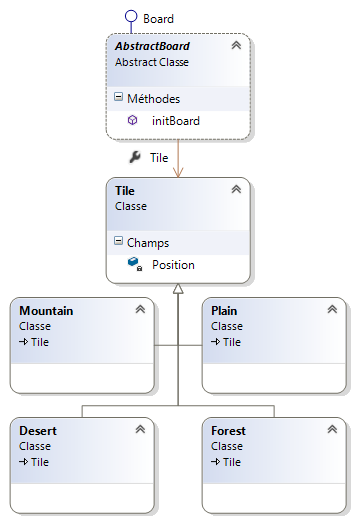
\includegraphics[width=0.3\textwidth]{img/PoidsMouche.png}
\caption{Exemple de patron de conception : poids-mouche}
\end{figure}

\subsection{Structure du code}

La structure de la partie "modèle" du code source est modelisée par le diagramme en annexe H. Il ne représente que la partie "Modèle" de l'architecture, les parties "Vue" et "Contrôleur" ne sont pas affichées.
Chaque joueur est représenté par une instance de la classe \emph{Player}.
La classe \emph{World} contiendra le plateau (avec la classe \emph{Board}), ainsi que les unités (instances de \emph{Unit}).
La classe \emph{Board} contiendra un ensemble de (avec la classe \emph{Tile}) qui représentent les différentes cases du terrain.

